\documentclass[french,]{compterendu}
\usepackage{lmodern}
\usepackage{amssymb,amsmath}
\usepackage{ifxetex,ifluatex}
\usepackage{fixltx2e} % provides \textsubscript
\ifnum 0\ifxetex 1\fi\ifluatex 1\fi=0 % if pdftex
  \usepackage[T1]{fontenc}
  \usepackage[utf8]{inputenc}
\else % if luatex or xelatex
  \ifxetex
    \usepackage{mathspec}
  \else
    \usepackage{fontspec}
  \fi
  \defaultfontfeatures{Ligatures=TeX,Scale=MatchLowercase}
\fi
% use upquote if available, for straight quotes in verbatim environments
\IfFileExists{upquote.sty}{\usepackage{upquote}}{}
% use microtype if available
\IfFileExists{microtype.sty}{%
\usepackage{microtype}
\UseMicrotypeSet[protrusion]{basicmath} % disable protrusion for tt fonts
}{}
\usepackage[left=2cm,right=2cm,top=2cm,bottom=2.5cm]{geometry}
\usepackage{hyperref}
\hypersetup{unicode=true,
            pdftitle={Projet Analyse de données},
            pdfauthor={Léo GABET},
            pdfkeywords={Langage python maos zencore},
            pdfborder={0 0 0},
            breaklinks=true}
\urlstyle{same}  % don't use monospace font for urls
\ifnum 0\ifxetex 1\fi\ifluatex 1\fi=0 % if pdftex
  \usepackage[shorthands=off,main=french]{babel}
\else
  \usepackage{polyglossia}
  \setmainlanguage[]{}
\fi
% Adding environment CSLReferences for compatibility with pandoc >= 2.8
% BEGIN

\newlength{\cslhangindent}
\setlength{\cslhangindent}{1.5em}
\newlength{\csllabelwidth}
\setlength{\csllabelwidth}{3em}
\newenvironment{CSLReferences}[2] % #1 hanging-ident, #2 entry spacing
 {% don't indent paragraphs
  \setlength{\parindent}{0pt}
  % turn on hanging indent if param 1 is 1
  \ifodd #1 \everypar{\setlength{\hangindent}{\cslhangindent}}\ignorespaces\fi
  % set entry spacing
  \ifnum #2 > 0
  \setlength{\parskip}{#2\baselineskip}
  \fi
 }%
 {}
\usepackage{calc} % for \widthof, \maxof
\newcommand{\CSLBlock}[1]{#1\hfill\break}
\newcommand{\CSLLeftMargin}[1]{\parbox[t]{\maxof{\widthof{#1}}{\csllabelwidth}}{#1}}
\newcommand{\CSLRightInline}[1]{\parbox[t]{\linewidth}{#1}}
\newcommand{\CSLIndent}[1]{\hspace{\cslhangindent}#1}

% END
\usepackage{longtable,booktabs}
\IfFileExists{parskip.sty}{%
\usepackage{parskip}
}{% else
\setlength{\parindent}{0pt}
\setlength{\parskip}{6pt plus 2pt minus 1pt}
}
\setlength{\emergencystretch}{3em}  % prevent overfull lines
\providecommand{\tightlist}{%
  \setlength{\itemsep}{0pt}\setlength{\parskip}{0pt}}
\setcounter{secnumdepth}{5}
% Redefines (sub)paragraphs to behave more like sections
\ifx\paragraph\undefined\else
\let\oldparagraph\paragraph
\renewcommand{\paragraph}[1]{\oldparagraph{#1}\mbox{}}
\fi
\ifx\subparagraph\undefined\else
\let\oldsubparagraph\subparagraph
\renewcommand{\subparagraph}[1]{\oldsubparagraph{#1}\mbox{}}
\fi

%%% Use protect on footnotes to avoid problems with footnotes in titles
\let\rmarkdownfootnote\footnote%
\def\footnote{\protect\rmarkdownfootnote}



%Mise en page
%\usepackage[left=2cm,right=2cm,top=2cm,bottom=2.5cm]{geometry}
%\usepackage{lastpage} %Pour numérotaion des pages
\usepackage{eso-pic} %pour l'image de fond de la page de garde
\usepackage{enumitem} %Pour personnaliser les listes à puces
\usepackage{fancyhdr}
\usepackage{xcolor}
\usepackage[T1]{fontenc}
\usepackage{amsthm}
%\usepackage{thmtools}

\usepackage[figure,table]{totalcount} % Pour avoir les nombres de figures, tables et théoremes
\usepackage{totcount} % Pour compter le nombre de références

%Gestion des tableaux
\usepackage{multirow}
\usepackage{float}
\floatplacement{table}{H}
\floatplacement{figure}{ht!}

%Divers
\usepackage{ifthen} %Gestion des instructions conditionnelles


\widowpenalty=10000
\clubpenalty=10000

%%%%%%%%%%%%%%%%%%%%%%%%%%%
%% Defining new counters %%
%%%%%%%%%%%%%%%%%%%%%%%%%%%

%% Compteur des références
\newtotcounter{citenum} 
\def\oldcite{}
\let\oldcite=\bibcite
\def\bibcite{\stepcounter{citenum}\oldcite}

\regtotcounter{figure}
\regtotcounter{table}
\regtotcounter{theorem}


%%%%%%%%%%%%%%%%%%%%%%%%%%%%%%%%%%%%%%%%%%%%%%%
%% Configuration des messages de type badbox %%
%%%%%%%%%%%%%%%%%%%%%%%%%%%%%%%%%%%%%%%%%%%%%%%

\widowpenalty=10000
\clubpenalty=10000


%%%%%%%%%%%%%%%%%%%%%%%%%%%%
%% Theorem environemments %%
%%%%%%%%%%%%%%%%%%%%%%%%%%%%


\theoremstyle{urcastyle}
\newtheorem{theorem}{Théorème}
\newtheorem{lemma}{Lemme}
\newtheorem{corollary}{Corollaire}
\newtheorem{proposition}{Proposition}
\newtheorem{definition}{Définition}
\newtheorem{example}{Exemple}

\theoremstyle{remark}
%\newtheorem*{proof}{Démonstration}


%%%%%%%%%%%%%%%%%%%%%%%%%%%%%%%%%%%%%%%%%%%%
%% Désignation des variables de la classe %%
%%%%%%%%%%%%%%%%%%%%%%%%%%%%%%%%%%%%%%%%%%%%

% Processing title
  \newcommand{\titlehead}{Projet Analyse de données}
  \title{Projet Analyse de données}
    % Processing authors
  \newcounter{nbaut}
  \setcounter{nbaut}{9} % Nombre d'auteurs
  \author{Léo GABET}
      \date{25 décembre 2023}

 \resume{BLABLA}
 \keywords{Langage python maos zencore.}

 \coefficient{50 \%}


  \email{\href{mailto:leo.gabet@etudiant.univ-reims.fr}{\nolinkurl{leo.gabet@etudiant.univ-reims.fr}}}
%\email{\href{mailto:leo.gabet@etudiant.univ-reims.fr}{\nolinkurl{leo.gabet@etudiant.univ-reims.fr}}}
\logouniv{logo_URCA.pdf}
\logoufr{logoSEN.pdf}
\date{25 décembre 2023}
\diplome{M2 SEP}
\anac{2023-2024}
\module{SEP0931}
\enseig{Emmanuelle Gauthérat}
\evaluation{PROJET ADD}

%% Passage des compteurs à la classe pour maketitle.
\totfig{\total{figure}}
\tottab{\total{table}}
\totref{\total{citenum}}
\tottheo{\total{theorem}}

%%%%%%%%%%%%%%%%%%%
%% Mise en forme %%
%%%%%%%%%%%%%%%%%%%


%Formatage en-têtes et pieds de pages
\pagestyle{fancy}
\fancyhead[L]{\small \titlehead}
%\fancyhead[C]{\small \textcolor{urcabrown}{\titlehead}}
\fancyhead[R]{}
\fancyfoot[l]{\small \ifnum\value{nbaut}=1 {\theauthor} \else {Léo GABET \textit{}\fi}}
\fancyfoot[C]{\small \it \theeval \ \themodule \ -- \theanac}
\fancyfoot[R]{\small \thepage\ / \pageref{LastPage}}
% \renewcommand{\headrule}{\hbox to\headwidth{%
%     \color{urcabrown}\leaders\hrule height \headrulewidth\hfill}}
% \renewcommand{\footrule}{\hbox to\headwidth{%
%     \color{urcabrown}\leaders\hrule height \headrulewidth\hfill}}
\renewcommand{\headrulewidth}{0.5pt}
\renewcommand{\footrulewidth}{0.5pt}

\renewcommand{\headrulewidth}{0.5pt}
\renewcommand{\footrulewidth}{0.5pt}

\fancypagestyle{plain}{%
\fancyhf{} % clear all header and footer fields
\fancyfoot[C]{\small \thepage\ / \pageref{LastPage}} % except the center
\renewcommand{\headrulewidth}{0pt}
\renewcommand{\footrulewidth}{0pt}}

\AtEndDocument{\thispagestyle{plain}}
% Pandoc header


%%%%%%%%%%%%%%%%%%%%%%%
%% Début du document %%
%%%%%%%%%%%%%%%%%%%%%%%

\begin{document}

\AddToShipoutPictureBG*{
\includegraphics[width=\paperwidth,height=\paperheight]{fond_a4_sen_3.pdf}}

% \theoremstyle{urca}
\newtheorem{lemme}{Lemme}[section]
\newtheorem{theoreme}{Théorème}[section]
% \newtheorem{proposition}{Proposition}[section]
% \newtheorem{definition}{Définition}[section]
\newtheorem{corollaire}{Corollaire}[section]
\newtheorem{propriete}{Propriété}[section]
\newtheorem{proprietes}{Propriétés}[section]



\maketitle

% \pagebreak
% 
% % \begin{abstract}
% BLABLA
% \end{abstract}
% 

\vspace{1cm}

  {
  \hypersetup{linkcolor=black}
  \setcounter{tocdepth}{2}
  \pagebreak
  \tableofcontents
  }

\pagebreak
\normalsize



\hypertarget{introduction}{%
\section{Introduction}\label{introduction}}

\hypertarget{contexte-de-luxe9tude}{%
\subsection{Contexte de l'étude}\label{contexte-de-luxe9tude}}

Le vélo est devenu un mode de transport de plus en plus populaire à travers le monde, offrant une alternative écologique et saine aux moyens de déplacement traditionnels. En France, l'a promotion de 'intérêt de l'utilisation du vélo est devenue une priorité, avec des efforts déployés pour créer des infrastructures adaptées, telles que des pistes cyclables, afin de favoriser la sécurité des cyclistes et encourager la pratique du vélo.

Cependant, malgré ces initiatives, la sécurité des cyclistes sur les routes reste une préoccupation majeure. Les accidents de vélos peuvent avoir des conséquences graves, mettant en lumière la nécessité d'une compréhension approfondie des facteurs contribuant à ces incidents. Dans ce contexte, l'analyse de données offre une approche précieuse pour examiner les tendances, les corrélations et les déterminants des accidents de vélos en France.

Cette analyse s'appuiera sur deux jeux de données différents. D'une part, une base de données détaillant les accidents de vélos survenus à travers le pays fournira des informations précieuses sur les circonstances, la gravité et les lieux des incidents. D'autre part, une base de données spécifique à Paris, décrivant la création et l'emplacement des pistes cyclables, permettra d'explorer la corrélation entre l'infrastructure dédiée aux cyclistes et la fréquence des accidents.

L'objectif de cette analyse est de dégager des tendances significatives, de mettre en évidence les zones à risque élevé, et d'évaluer l'impact des pistes cyclables sur la sécurité des cyclistes. En comprenant les facteurs sous-jacents aux accidents de vélos, il devient possible d'orienter les politiques publiques, d'améliorer les infrastructures et de promouvoir des mesures préventives pour garantir une cohabitation sûre et efficace entre les cyclistes et les autres usagers de la route.

Cette étude contribuera ainsi à la promotion d'une mobilité durable, en mettant en lumière les défis actuels et en proposant des solutions basées sur des données probantes pour renforcer la sécurité des cyclistes en France.

\hypertarget{plan-de-luxe9tude}{%
\subsection{Plan de l'étude}\label{plan-de-luxe9tude}}

En exploitant les données nationales disponibles sur le site \textbf{data gouv}, notre première étape consistera à dégager les tendances des accidents de vélos et à localiser les zones à risques élevés à l'échelle nationale. Cette analyse globale sera ensuite approfondie par un zoom sur Paris, permettant ainsi de cerner les défis spécifiques rencontrés dans la capitale.

La deuxième phase de notre étude se concentrera sur l'analyse de la base de données détaillant les pistes cyclables à Paris ici du site \textbf{data Paris}. Cette démarche vise à cartographier ces infrastructures et à examiner leur évolution au fil du temps. Comprendre ces dynamiques est essentiel pour évaluer l'influence de l'infrastructure sur la sécurité des cyclistes.

Enfin, nous croiserons les données d'accidents par arrondissement avec la présence de pistes cyclables. Cette approche nous permettra de déterminer les liens entre les accidents de vélos et l'existence de pistes cyclables. L'objectif ultime est d'identifier des zones spécifiques nécessitant des améliorations ciblées afin de renforcer la sécurité des cyclistes dans la ville de Paris.

\hypertarget{donnuxe9es}{%
\section{Données}\label{donnuxe9es}}

Les jeux de données comprennent une couverture complète des accidents de vélo à l'échelle nationale en France, offrant une vue d'ensemble des incidents survenus dans tout le pays. Un second jeu de données se concentre spécifiquement sur les pistes cyclables, cartographiant l'infrastructure dédiée dans diverses localités. Enfin, un troisième jeu de données se focalise sur les accidents de vélo à Paris, avec des informations détaillées sur les arrondissements. Ces ensembles de données permettent d'analyser les tendances, de localiser les zones à risques et d'évaluer l'impact des pistes cyclables sur la sécurité, offrant ainsi une compréhension approfondie de la situation des cyclistes en France.

\hypertarget{analyse-des-accidents-de-vuxe9los-en-france}{%
\section{Analyse des Accidents de Vélos en France}\label{analyse-des-accidents-de-vuxe9los-en-france}}

\hypertarget{exploration-des-bases-de-donnuxe9es-sur-les-accidents-de-vuxe9los-uxe0-luxe9chelle-nationale}{%
\subsection{Exploration des bases de données sur les accidents de vélos à l'échelle nationale}\label{exploration-des-bases-de-donnuxe9es-sur-les-accidents-de-vuxe9los-uxe0-luxe9chelle-nationale}}

\begin{figure}[H]

{\centering 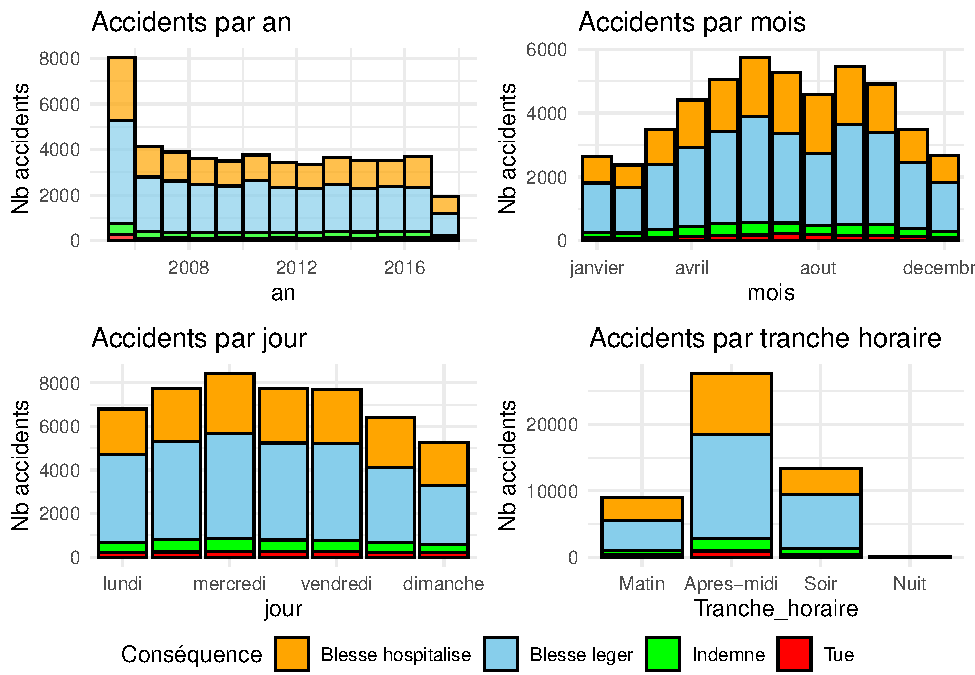
\includegraphics[width=1\linewidth]{Rapport_ADD_LEO-GABET_files/figure-latex/accfrancedetail-1} 

}

\caption{Représentation des accidents de vélo en France par année, mois, jour et horaire}\label{fig:accfrancedetail}
\end{figure}

Les accidents de vélos se déroulent principalement durant les mois à température douce voir chaude, tel que le mois de juin qui représente un pic des accidents de vélos sur 13 ans.
On contaste bien que le type de jour lié aux accidents correspond aux jours de la semaine, avec une très grande part d'accident lors des après-midi.

\hypertarget{identification-des-zones-uxe0-risques-uxe9levuxe9s-uxe0-luxe9chelle-du-pays}{%
\subsection{Identification des zones à risques élevés à l'échelle du pays}\label{identification-des-zones-uxe0-risques-uxe9levuxe9s-uxe0-luxe9chelle-du-pays}}

\begin{figure}[H]

{\centering 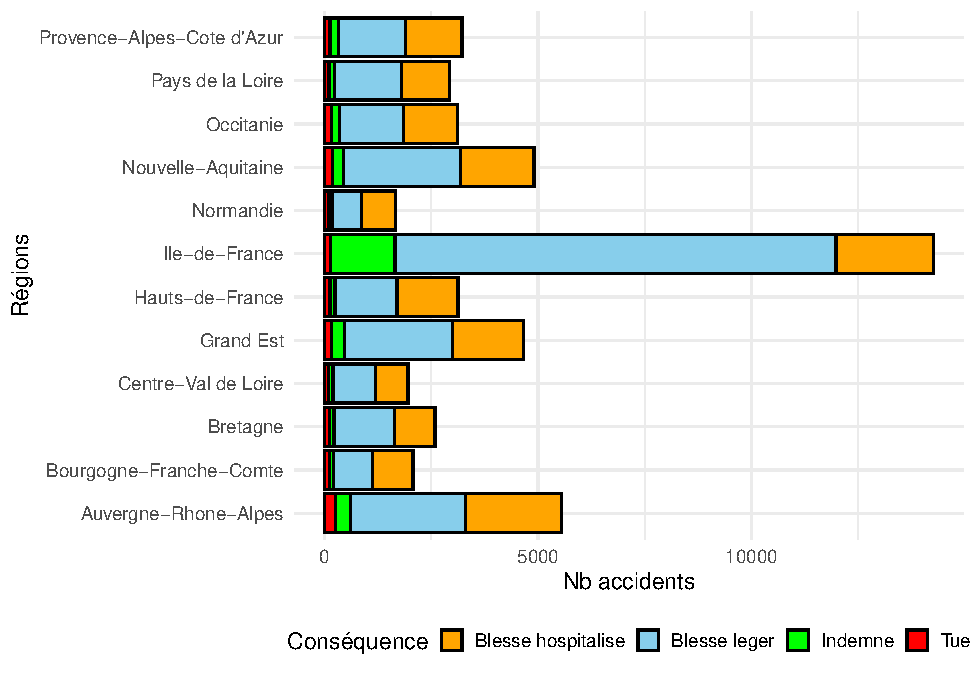
\includegraphics[width=1\linewidth]{Rapport_ADD_LEO-GABET_files/figure-latex/accfranceregion-1} 

}

\caption{Accidents en France en fonction des régions}\label{fig:accfranceregion}
\end{figure}

Une grande partie des accidents de vélo en France se déroule principalement en île de France, avec une très faible présence d'accidence en Provence-Alpes-Cote d'Azur (et Corse).

\hypertarget{facteurs-et-contextes}{%
\subsection{Facteurs et contextes}\label{facteurs-et-contextes}}

\begin{figure}[H]

{\centering 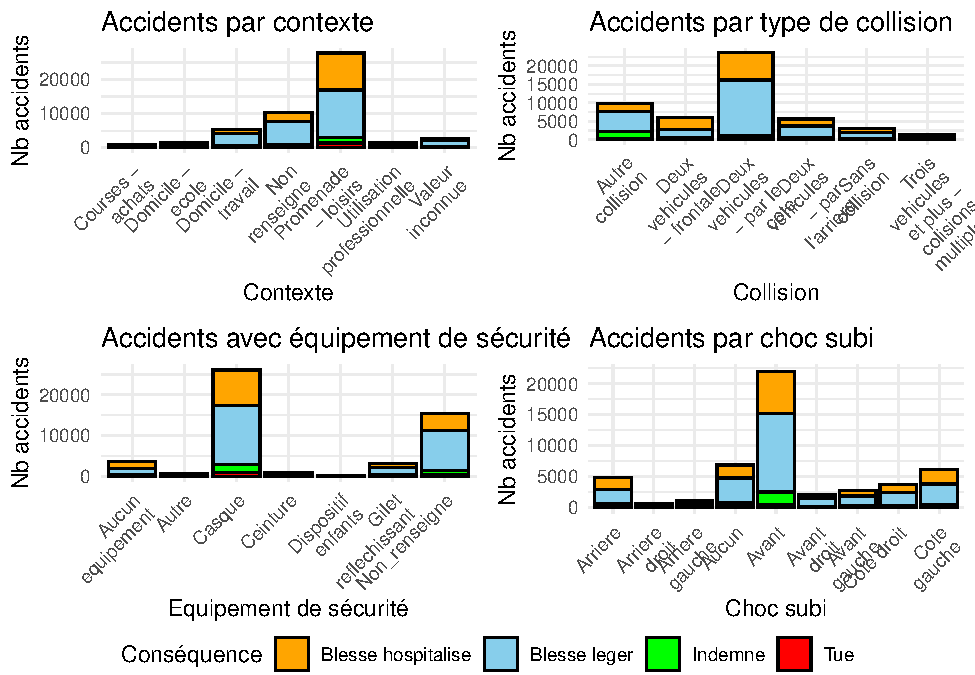
\includegraphics[width=1\linewidth]{Rapport_ADD_LEO-GABET_files/figure-latex/accCONTEXTE-1} 

}

\caption{Représentation des accidents de vélo en France par les contextes des collisions et choc subi avec les équipements de sécurités}\label{fig:accCONTEXTE}
\end{figure}

C'est lors de promenade et loisirs que les accidents de vélos se produisent le plus souvent, notamment par les voitures sur les cotés provoquant pour la plus part des chocs avant. On relève néanmoins que la plus part des accidentés possèdent au minima un casque pour leur équipement de sécurité, ce qui pourrait expliqué la forte présence de la conséquence ``blessé léger''.

\hypertarget{zoom-sur-paris-analyse-duxe9tailluxe9e-des-accidents-dans-la-capitale}{%
\subsection{Zoom sur Paris : Analyse détaillée des accidents dans la capitale}\label{zoom-sur-paris-analyse-duxe9tailluxe9e-des-accidents-dans-la-capitale}}

\begin{figure}[H]

{\centering 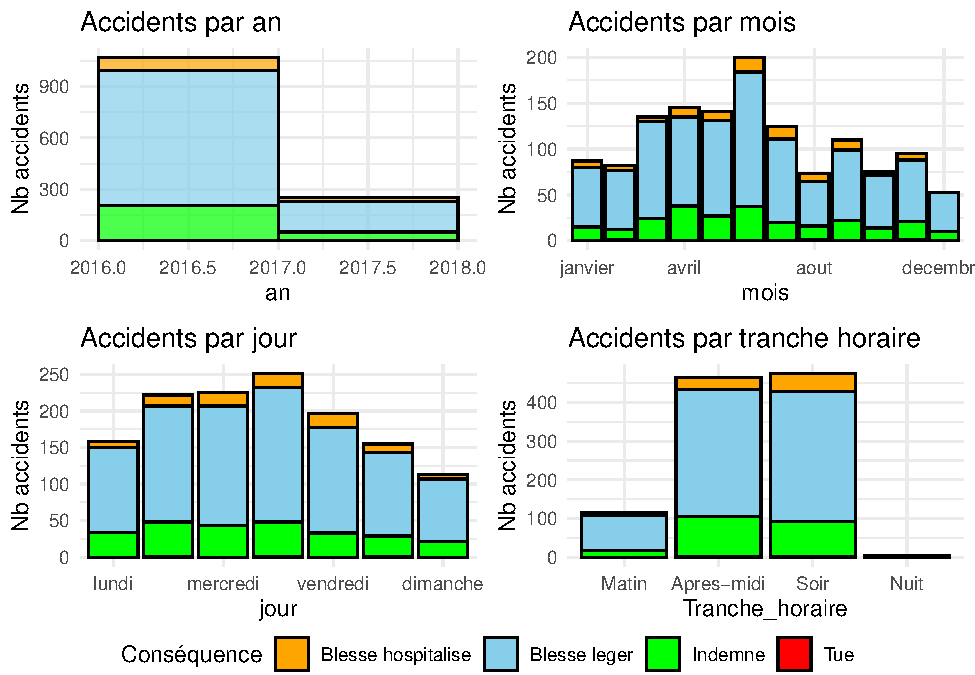
\includegraphics[width=1\linewidth]{Rapport_ADD_LEO-GABET_files/figure-latex/accParisdetail-1} 

}

\caption{Représentation des accidents de vélo à Paris par année, mois, jour et horaire}\label{fig:accParisdetail}
\end{figure}

Nous allons nous concentré sur les années 2016, 2017 et 2018 qui représentent un très grand nombre d'accident pour Paris.

\hypertarget{infrastructures-cyclables-uxe0-paris}{%
\section{Infrastructures Cyclables à Paris}\label{infrastructures-cyclables-uxe0-paris}}

\hypertarget{introduction-de-la-base-de-donnuxe9es-sur-les-pistes-cyclables-uxe0-paris}{%
\subsection{Introduction de la base de données sur les pistes cyclables à Paris}\label{introduction-de-la-base-de-donnuxe9es-sur-les-pistes-cyclables-uxe0-paris}}

Avant d'étudier

\hypertarget{uxe9tude-des-variations-dans-la-cruxe9ation-des-pistes-cyclables-au-fil-du-temps}{%
\subsection{Étude des variations dans la création des pistes cyclables au fil du temps}\label{uxe9tude-des-variations-dans-la-cruxe9ation-des-pistes-cyclables-au-fil-du-temps}}

\begin{figure}[H]

{\centering 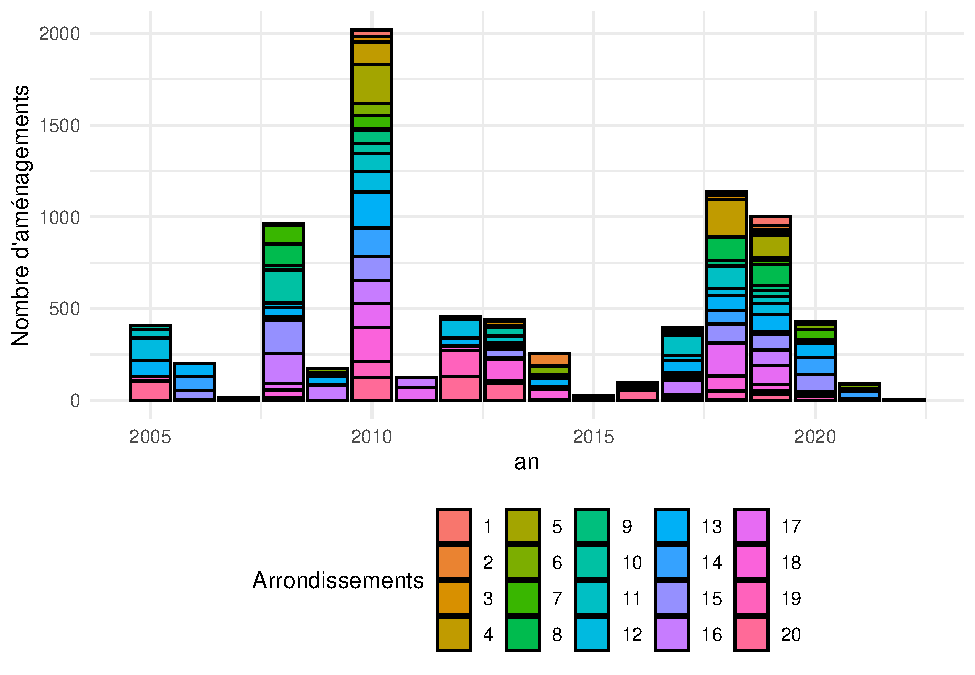
\includegraphics[width=1\linewidth]{Rapport_ADD_LEO-GABET_files/figure-latex/arrPARISdetails-1} 

}

\caption{Évolution des pistes cyclables dans les arrondissements au fil des années}\label{fig:arrPARISdetails}
\end{figure}

On remarqu'en 2010, beaucoup d'aménagement ont été effecuté dans l'ensemble des arrondissements de Paris. Cependant, on constate que le deuxième arrondissement possède le moins d'aménagement de piste cyclable ! De plus, pas mal de travaux d'aménagement ont lieu entre 2016 et 2019, ce qui pourrai expliqué la présence d'un pic d'accident de vélo dans Paris étant donné que les cyclistes n'avaient donc pas de pistes cyclables de présent pour rouler dessus.

\begin{figure}[H]

{\centering 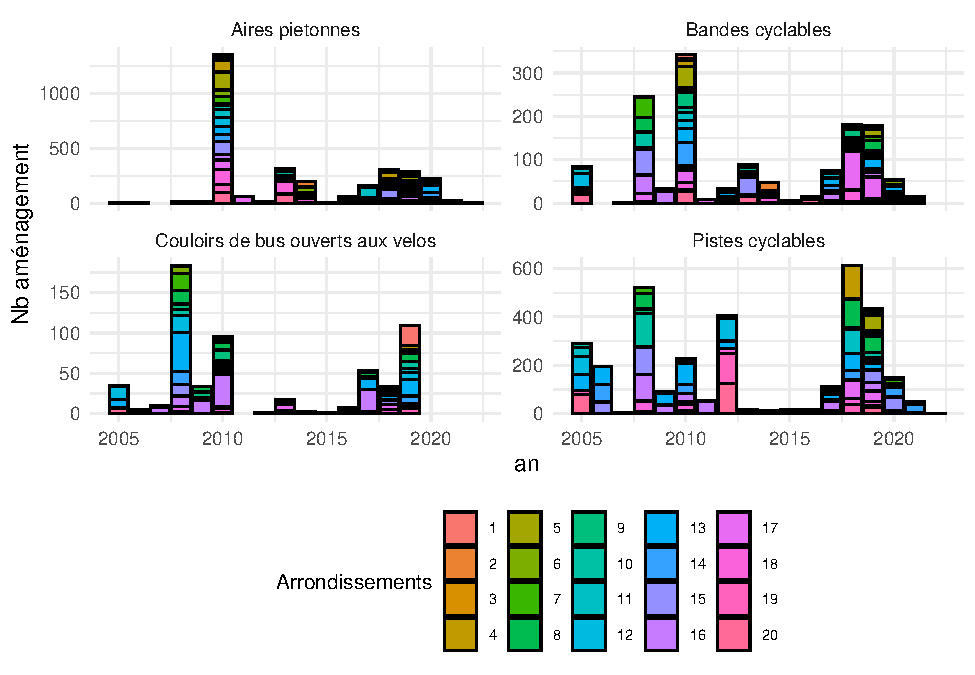
\includegraphics[width=1\linewidth]{Rapport_ADD_LEO-GABET_files/figure-latex/arrPARISTypo-1} 

}

\caption{Évolution des typologies selon les arrondissements au fil des années}\label{fig:arrPARISTypo}
\end{figure}

On voit donc que selon les différentes typologies d'aménagements où les vélos peuvent circulés, les pistes et bandes cyclables dominent, avec encore une fois par exemple le faite que le deuxième arrondissement possède le moins d'aménagement pour les vélos.

\hypertarget{croisement-des-donnuxe9es-accidents-et-pistes-cyclables-uxe0-paris}{%
\section{Croisement des Données : Accidents et Pistes Cyclables à Paris}\label{croisement-des-donnuxe9es-accidents-et-pistes-cyclables-uxe0-paris}}

\hypertarget{agruxe9gation-des-donnuxe9es-daccidents-par-arrondissement-uxe0-paris}{%
\subsection{Agrégation des données d'accidents par arrondissement à Paris}\label{agruxe9gation-des-donnuxe9es-daccidents-par-arrondissement-uxe0-paris}}

\begin{figure}[H]

{\centering 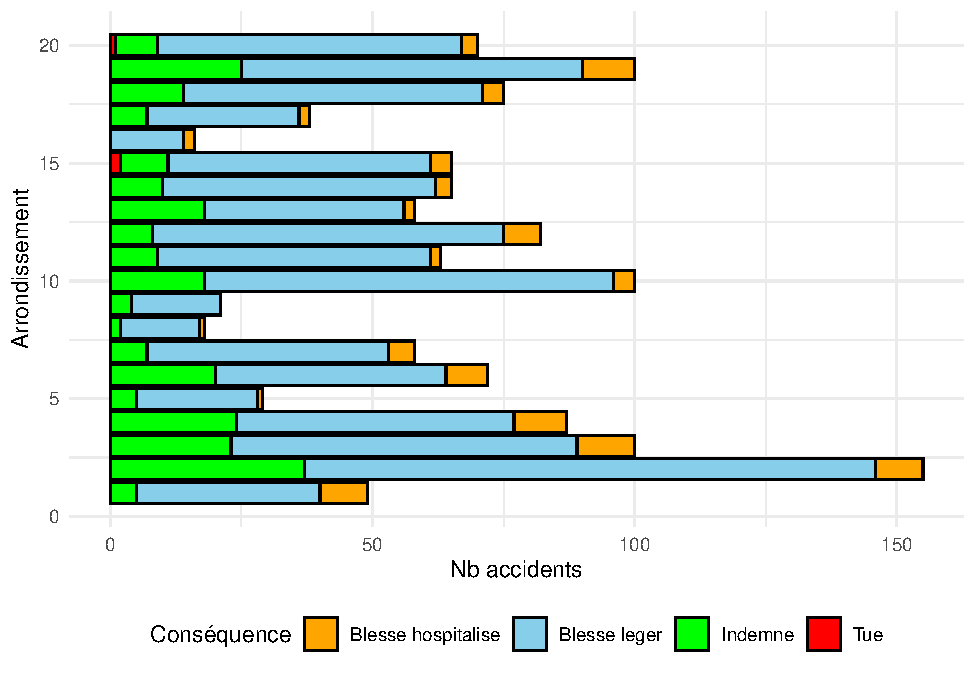
\includegraphics[width=1\linewidth]{Rapport_ADD_LEO-GABET_files/figure-latex/arrPARISaccident-1} 

}

\caption{Les accidents de vélos selon les arrondissements de Paris}\label{fig:arrPARISaccident}
\end{figure}

\hypertarget{analyse-des-liens-entre-les-accidents-de-vuxe9los-et-la-pruxe9sence-de-pistes-cyclables}{%
\subsection{Analyse des liens entre les accidents de vélos et la présence de pistes cyclables}\label{analyse-des-liens-entre-les-accidents-de-vuxe9los-et-la-pruxe9sence-de-pistes-cyclables}}

\hypertarget{identification-des-arrondissements-pruxe9sentant-des-duxe9fis-particuliers-ou-des-amuxe9liorations-nuxe9cessaires}{%
\subsection{Identification des arrondissements présentant des défis particuliers ou des améliorations nécessaires}\label{identification-des-arrondissements-pruxe9sentant-des-duxe9fis-particuliers-ou-des-amuxe9liorations-nuxe9cessaires}}

Sans surprise, le deuxième arrondissement possède la majorité des accidents de vélos suivi des 3ième, 10ième, 19ième et 20ième arrondissements. Concernant le 2ième arrondissement, une simple hypothèse viendrait du faite qu'il s'agit du centre même de Paris, donc la localisation qui regroupe le plus de personnes ! et d'autre part, nous avons aussi vu que le nombre d'aménagement étaient très bas dans cet arrondissement.

\hypertarget{conclusion}{%
\section{Conclusion}\label{conclusion}}

\hypertarget{annexes}{%
\section{Annexes}\label{annexes}}

\hypertarget{base-de-donnuxe9es}{%
\subsection{Base de données}\label{base-de-donnuxe9es}}

Mettre ici les natures des variables

\hypertarget{analyse-univariuxe9}{%
\subsection{Analyse univarié}\label{analyse-univariuxe9}}

\hypertarget{analyse-bivariuxe9}{%
\subsection{Analyse bivarié}\label{analyse-bivariuxe9}}

\hypertarget{analyse-multivariuxe9}{%
\subsection{Analyse multivarié}\label{analyse-multivariuxe9}}




\end{document}
